A large part of the design of a legged robot depends on the design of a simple leg - more specifically the degrees of freedom that a single leg has. The degrees of freedom that a single leg has is determined by the amount of dimensions that the leg can make a controlled movement in, independently from any other dimensions. There are two common underlying designs in robot leg design - these are for two and three degrees of freedom respectively.\\

Figure \ref{fig:2DOF} shows an example of a common design that has two degrees of freedom. The design therefore contains two joints in one leg. In this example, the first joint is positioned vertically to form the hip op the robot leg. This allows for the side to side motion required for walking. The second joint is positioned horizontally to allow the lowest limb to move up and down. The two degrees of freedom controlled by this leg design is therefore the horizontal angle of the leg and the height of the foot. These two (and only these two) parameters therefore can be controlled completely independently.
\FloatBarrier
\begin{figure}[h]
\centering
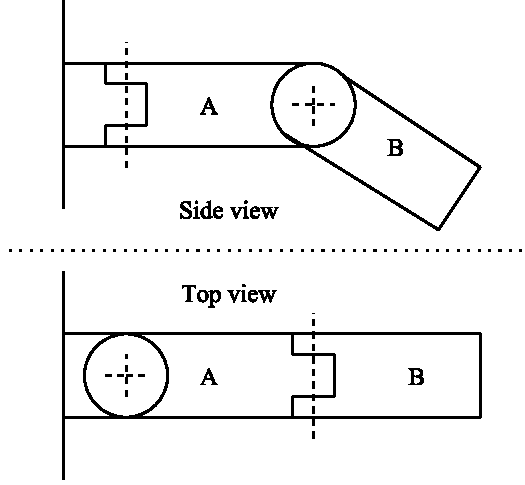
\includegraphics[scale = 1]{pics/2DOF.pdf}
\caption{Example of a leg design with two degrees of freedom.}
\label{fig:2DOF}
\end{figure}
\FloatBarrier
An example of a robotic leg with three degrees of freedom can be seen in Figure \ref{fig:3DOF}. This design is similar to that of the leg with two degrees of freedom seen in Figure \ref{fig:2DOF}, with the only addition being a second horizontal joint further down from the first. This additional limb means that the horizontal distance from the foot to the hip can be controlled as well as the height of the foot. These two controlled parameters together with the horizontal leg angle which can also be controlled independently as in the case of the two degrees of freedom design means that this design has a total of three degrees of freedom.
\FloatBarrier
\begin{figure}[h]
\centering
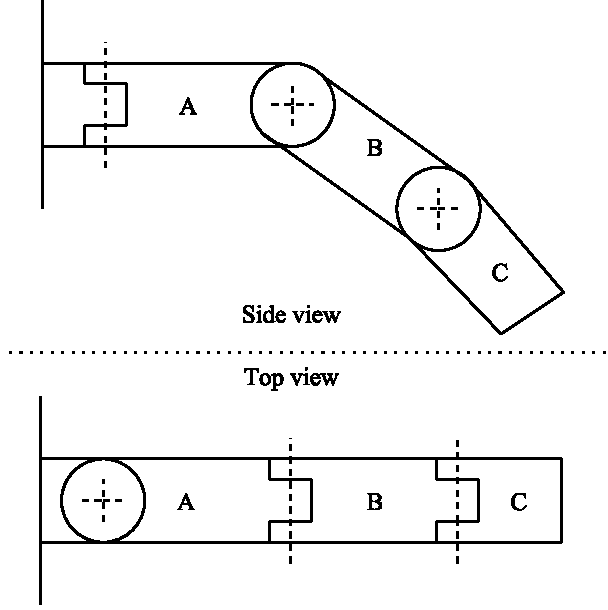
\includegraphics[scale = 1]{pics/3DOF.pdf}
\caption{Example of a leg design with three degrees of freedom.}
\label{fig:3DOF}
\end{figure}
\FloatBarrier
The overall shape of the robot and, more specifically, the placement of legs around the robot will greatly influence the robot's performance when moving forward in a straight line, moving sideways and moving over obstacles.

A popular design in hexapod robots is placing the legs in groups of three on opposite sides. This means that the legs are all aligned in a similar direction while the body is usually a long rectangular shape, similar to that found on insects. The advantage of this design lies mainly in the ability to move forward very quickly since the legs are placed optimally for forward motion. While holonomic movement is possible, it is usually much slower than forward or backward motion. This design is usually more suited to robots with an even number of legs due to the symmetry of the design. An example of such a configuration is illustrated in Figure \ref{fig:Body_layout_hex}.
\FloatBarrier
\begin{figure}[h]
\centering
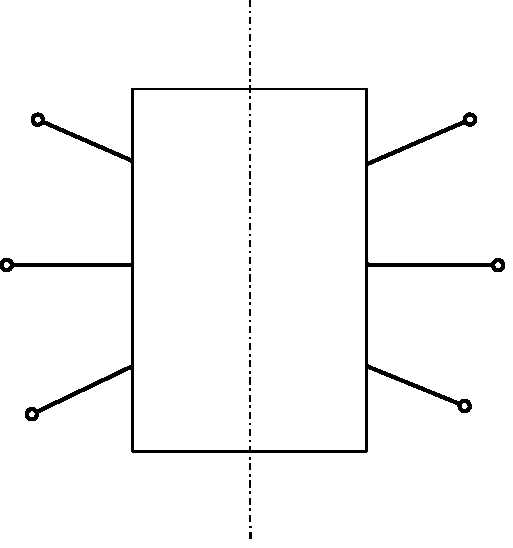
\includegraphics[scale = 1]{pics/Body_layout_hex.pdf}
\caption{Example of a symmetric hexapod robot chassis.}
\label{fig:Body_layout_hex}
\end{figure}
\FloatBarrier

An alternative design approach is to space the legs evenly around the robot chassis. The robot chassis would normally be round or a polygon with the same number of sides as legs. In the case of a five legged robot, the legs would be positioned $\frac{360^o}{5} = 72^o $ apart.
This equally spaced design approach has the disadvantage of not being particularly fast in any given direction but the advantage that it can manage the maximum speed in any given direction. Figure \ref{fig:Body_layout} shows an example of a circular body with five equally spaced legs. 

\FloatBarrier
\begin{figure}[h]
\centering
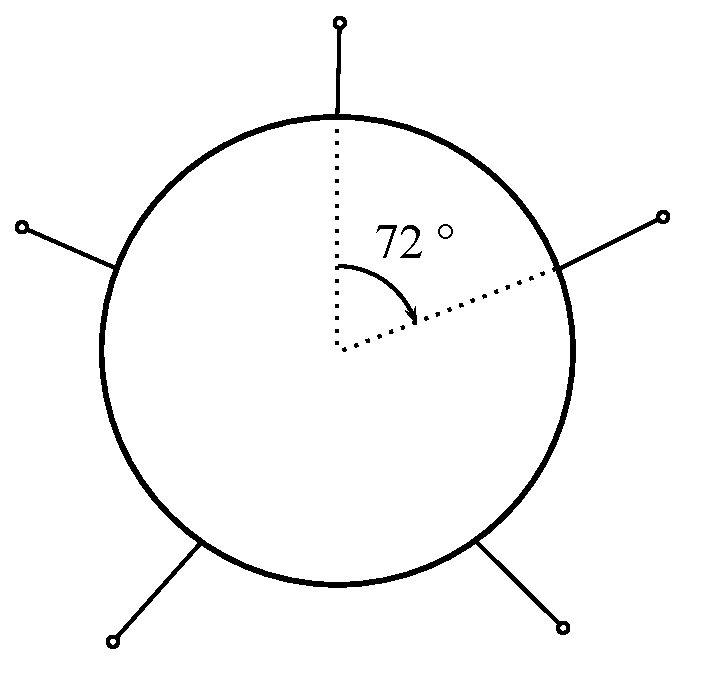
\includegraphics[scale = 1]{pics/Body_Layout.pdf}
\caption{Example of a robot chassis with equally spaced legs.}
\label{fig:Body_Layout}
\end{figure}
\FloatBarrier

Choosing actuators for the movement of the legs will determine how well the robot functions, how complicated the implementation is, how battery life is impacted and what type of feedback is required. The three types of motors considered is geared DC motors, stepper motors and servo motors.

Geared DC motors are simple to implement mechanically because small motor assemblies can often have a high torque output because of the integrated gearbox. The disadvantage of using a gearbox is that it can make the response sluggish if the reduction ratio is too high. Motor speed can easily be controlled by using pulse width modulation (PWM) to control the current through the motor. It is much more difficult to control motor position. In order to make a functioning control system with this type of motor, some feedback is required on the current position (shaft angle) of the motor. This can be implemented with a rotary encoder or in the case where the shaft never makes a full rotation, a potentiometer. The control system can then apply the voltage necessary to the motor in order to reach the required angular position. It will be necessary to apply negative voltages to the motor in some cases to make it reverse. The simplest way to achieve this is by implementing the motor control circuit with an H-bridge.

Stepper motors move in discrete steps and it is therefore much simpler to keep track of shaft angle and calculate the steps required to reach a given angle if the current angle is known. In order to know where it is when turned on, servo motors are often implemented with a 'home' position it can use as reference. This requires some sensor used to determine if the arm is in a specific position or not. A homing routine is used when initializing the robot wherein the robot moves a limb with unknown position in a specific direction while continuously polling the homing sensor for change. As soon as the sensor senses the presence of the arm, movement is seized and the current position is determined to be the home position. All movements can then be calculated from this reference position

The design with three degrees of freedom has the advantage of being able to lift a leg without altering the horizontal position of the leg. This means that the robot is able to walk without altering the height of the body of the robot. This means that the robot is able to much better cross rougher terrain because of the ability to alter the height the robot feet as the terrain requires. With the design that has two degrees of freedom, the foot height is a function of the horizontal extension of the leg. With this design the main advantage is the simplicity - both mechanically and in software. The cost and power consumption will also be much lower because of the reduced amount of actuators.\\

Due to the much greater flexibility of the design with three degrees of freedom and the ability to cross rougher terrain, this will be the platform implemented in the final design.\\

Since this robot is being designed specifically for holonomic movement and has an odd number of legs, another design might be more suited.